
In the sequential data structures we have studied so far, the data is stored in an array (or at least a conceptual array made up of memory blocks). Now we will consider a very different type of data structure where the data is linked together by pointers. The simplest example is a list where each element is allocated separately, but everything we learn here applies to other nodal containers such as trees, graphs, or any other data structure where each element is allocated separately, and the data is linked together by pointers.

For simplicity, we will consider a singly linked list; in STL, it is available as std::forward\_list:

\hspace*{\fill} \\ %插入空行
\begin{center}
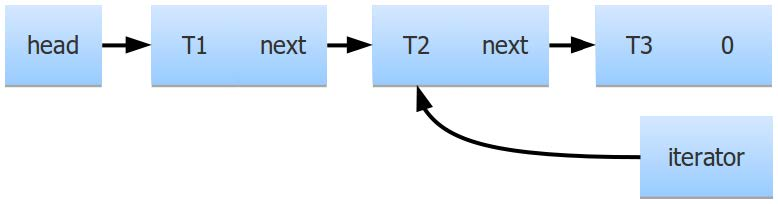
\includegraphics[width=0.9\textwidth]{content/2/chapter7/images/24.jpg}\\
Figure 7.24 – Singly-linked list with iterators
\end{center}

Because each element is allocated separately, it can also be deallocated individually. Often, a lightweight allocator is used for these data structures, where the memory is allocated in large blocks that are partitioned into node-sized fragments. When a node is deallocated, the memory is not returned to the OS but is put on a free list for the next allocation request. For our purposes, it is largely irrelevant whether the memory is allocated directly from the OS or handled by a specialized allocator (although the latter can often be much more efficient).

The list iterators present an additional challenge in concurrent programs. As we see in Figure 7.24, these iterators can point anywhere in the list. If an element is removed from the list, we expect its memory to eventually become available for constructing and inserting another element (if we do not do this and hold all memory until the entire list is deleted, adding and removing a few elements repeatedly can waste a lot of memory). However, we cannot delete the list node if there is an iterator pointing to it. This is true in single-threaded programs as well, but it is often much harder to manage in concurrent programs. With multiple threads possibly working with iterators, we often cannot guarantee by the execution flow of the operations that no iterators are pointing to the element we are about to delete. In this case, we need the iterators to extend the lifetime of the list nodes that they point to. This, of course, is a job for reference-counted smart pointers such as std::shared\_ptr. Let's assume from now on that all the pointers in the list, both the ones linking the nodes together and the ones inside the iterators, are smart pointers (std::shared\_ptr or a similar pointer with stronger thread-safety 
guarantees).

Just like we did with the sequential data structures, our first attempt at a thread-safe data structure should be a lock-guarded implementation. In general, you should never design a lock-free data structure until you know that you need one: developing lock-free code may be cool, but trying to find bugs in it is most definitely not. 

Just like we did earlier, we have to redesign parts of the interface, so all operations are transactional: pop\_front() should work whether the list is empty or not, for example. We can then protect all operations with a lock. For operations such as push\_front() and pop\_front(), we can expect a performance similar to what we have observed for the stack or the queue earlier. But the list presents additional challenges we did not have to face until now. 

First, the list supports insertions at arbitrary locations; in the case of std::forward\_list, it is inser\_after() to insert a new element after the one pointed to by an iterator. If we insert two elements on two threads simultaneously, we would like the insertions to proceed concurrently unless the two locations are close to each other and affect the same list node. But we cannot get that with a single lock guarding the entire list. 

The situation is even worse if we consider long-running operations such as searching the list for an element that has the desired value (or satisfies some other condition). We would have to lock the list for the entire search operation, so no adding or removing elements to the list while the list is traversed. Of course, if we search frequently, the list is not the right data structure, but trees and other nodal data structures have the same problem: if we need to traverse large parts of the data structure, the lock is held for the duration of the entire operation, preventing all other threads from accessing even the nodes unrelated to the ones we're currently operating on.

Of course, these problems are not your concern if you never encounter them: if your list is accessed from the front and backends only, then a lock-guarded list may be perfectly sufficient. As we have seen many times, when it comes to designing concurrent data structures, unnecessary generality is your enemy. Build only what you need.

Most of the time, however, nodal data structures are accessed not just from the ends or, in the case of trees or graphs, there aren't really any ends. Locking the entire data structure so that it can be accessed by only one thread at a time is not acceptable if the program spends most of the time operating on this data structure. The next idea you may consider is locking each node separately; in the case of the list, we could add a spinlock to every node and lock the node if we need to change it. Unfortunately, this approach runs into the problem that is the bane of all lock-based solutions: the deadlocks. Any thread that needs to operate on more than one node will have to acquire multiple locks. Let's say that thread A holds the lock on node 1, and now it needs to insert a new node after node 2, so it tries to get that lock too. At the same time, thread B holds the lock on node 2, and it wants to erase the node after node 1, so it tries to get that lock. Both threads will now wait forever. This problem is not avoidable with so many locks that can be acquired in arbitrary order unless we enforce very strict limitations on how the threads may access the list (hold only one lock at any time), and then we run the risk of livelocks as many threads constantly release and reacquire locks.

If we truly need a list or another nodal data structure that is accessed concurrently, we have to come up with a lock-free implementation. As we have seen already, lock-free code is not easy to write and even harder to write correctly. Quite often, the better option is to come up with a different algorithm that does not require a thread-safe nodal data structure. Often, this can be done by copying parts of the global data structure into a thread-specific one that is then accessed by a single thread; at the end of the computation, the fragments from all threads are put together again. Sometimes, it is easier to partition the data structure so no nodes are accessed concurrently (for example, it may be possible to partition the graph and process each subgraph on one thread and then handle the boundary nodes). But if you really need a thread-safe nodal data structure, the next section will explain the challenges and give you some options for the implementation.

\subsubsubsection{7.5.1\hspace{0.2cm}Lock-free list}

The basic idea behind a lock-free list, or any other nodal container, is quite simple and is based on using compare-and-swap to manipulate the pointers to the nodes. Let's start with the simpler operation: the insertion. We are going to describe the insertion at the head of the list, but the insertion after any other node works the same way. 

\hspace*{\fill} \\ %插入空行
\begin{center}
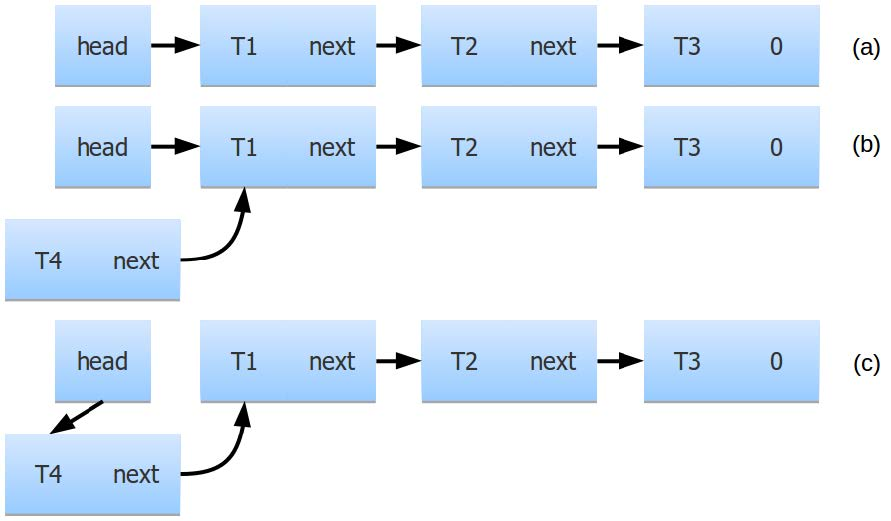
\includegraphics[width=0.9\textwidth]{content/2/chapter7/images/25.jpg}\\
Figure 7.25 – Insertion of a new node at the head of a singly-linked list
\end{center}

Let's say that we want to insert a new node at the head of the list shown in Figure 7.25a. The first step is to read the current head pointer, that is, the pointer to the first node. Then we create the new node with the desired value; its next pointer is the same as the current head pointer, so this node is linked into the list before the current first node (Figure 7.25b). At this point, the new node is not yet accessible to any other thread, so the data structure can be accessed concurrently. Finally, we execute the CAS: if the current head pointer is still unchanged, we atomically replace it with the pointer to the new node (Figure 7.25c). If the head pointer no longer has the value it had when we first read it, we read the new value, write it as the next pointer of our new node, and try the atomic CAS  again.

This is a simple and reliable algorithm. It is the generalization of the publishing protocol we saw in the previous chapter: the new data is created on a thread with no concern for thread safety because it is not yet accessible to other threads. As the final action, the thread publishes the data by atomically changing the root pointer from which all the data can be accessed (in our case, the head of the list). If we were inserting the new node after another node, we would atomically change that node's next pointer instead. The only difference is that multiple threads may be trying to publish new data at the same time; to avoid data races, we have to use compare-and-swap. 

Now, let's consider the opposite operation, erasing the front node of the list. This is also done in three steps:

\hspace*{\fill} \\ %插入空行
\begin{center}
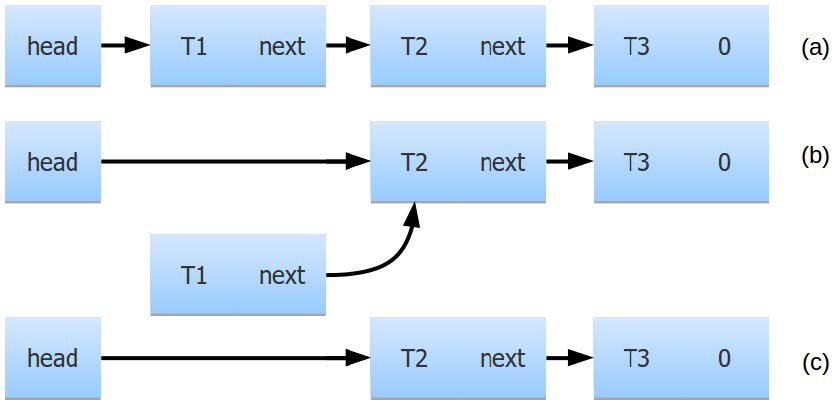
\includegraphics[width=0.9\textwidth]{content/2/chapter7/images/26.jpg}\\
Figure 7.26 – Lock-free removal at the head of a singly-linked list
\end{center}

First, we read the head pointer, use it to access the first node of the list, and read its next pointer (Figure 7.26a). Then we atomically write the value of that next pointer into the head pointer (Figure 7.26b), but only if the head pointer has not changed (CAS). At this point, the former first node is not accessible to any other thread, but our thread still has the original value of the head pointer and can use it to delete the node we had removed (Figure 7.26c). This is, again, simple and reliable. But the trouble arises when we try to combine both of these operations. 

Let's assume that two threads operate on the list at the same time. Thread A is trying to remove the first node of the list. The first step is to read the head pointer and the pointer to the next node; this pointer is about to become the new head of the list, but the compare-and-swap hasn't happened yet. For now, the head is unchanged, and the new head is a value head' that exists only in some local variable of thread A. This moment is captured in Figure 7.27a:

\hspace*{\fill} \\ %插入空行
\begin{center}
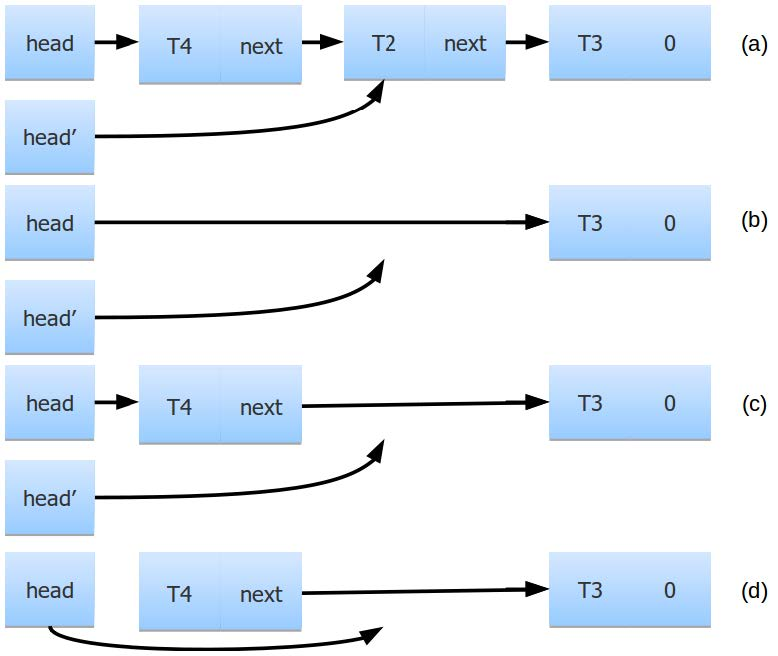
\includegraphics[width=0.9\textwidth]{content/2/chapter7/images/27.jpg}\\
Figure 7.27 – Lock-free insertion and removal at the head of a singly-linked list
\end{center}

Just at this moment, thread B successfully removes the first node of the list. Then it removes the next node also, leaving the list in the state shown in Figure 7.27b (thread A has not made any more progress). Thread B then inserts a new node at the head of the list (Figure 7.27c); however, since the memory of the two deleted nodes was deallocated, the new allocation for the node T4 reuses the old allocation, so the node T4 is allocated at the same address as the original node T1 used to have. This can easily happen as long as the memory of the deleted nodes is available for new allocations; in fact, most memory allocators prefer to return the most recently released memory on the assumption that it is still hot in the cache of the CPU.

Now, thread A is finally running again, and the operation it is about to do is compare-and-swap: if the head pointer has not changed since the last time thread A read it, the new head becomes head'. Unfortunately, the value of the head pointer is still the same, as far as thread A can see (it could not observe the entire history of the changes). The CAS operation succeeds, and the new head pointer now points to the unused memory where the node T2 used to be, while the node T4 is no longer accessible (Figure 7.27d). The entire list is corrupted.

This failure mechanism is so common in lock-free data structures that it has a name: the A-B-A problem. A and B here refer to memory locations: the problem is that some pointer in the data structure changes its value from A to B and then back to A. Another thread observes only the initial and the final values and sees no change at all; the compare-and-swap operation succeeds, and the execution takes the path where the programmer has assumed that the data structure is unchanged. Unfortunately, this assumption is not true: the data structure may have changed almost arbitrarily, except that the value of the observed pointer was restored to what it once was. 

The root of the problem is that if the memory is deallocated and reallocated, pointers, or addresses in memory, do not uniquely identify the data stored at that address. There are multiple solutions to this problem, but they all accomplish the same thing by different means: you have to make sure that once you read a pointer that will eventually be used by compare-and-swap, the memory at that address cannot be deallocated until the compare-and-swap is done (successfully or otherwise). If the memory is not deallocated, then another allocation cannot happen at the same address, and you are safe from the A-B-A problem. Note that not deallocating memory is not the same as not deleting nodes: you can certainly make the node inaccessible from the rest of the data structure (remove the node), and you can even call the destructor for the data stored in the node; you just  cannot free the memory occupied by the node. 

There are many ways to solve the A-B-A problem by delaying memory deallocation. The application-specific options are usually the simplest if they are possible. If you know that the algorithm does not remove many nodes over the lifetime of the data structure, you may simply keep all removed nodes on a list of deferred deallocations, to be deleted when the entire data structure is deleted. A more general version of this approach can be described as application-driven garbage collection: all deallocated memory goes on a garbage list first. The garbage memory is periodically returned to the main memory allocator, but during this garbage collection, all operations on the data structure are suspended: the operations in progress must complete before the collection starts, and all new operations are blocked until the collection is done. This ensures that no compare-and-swap operation can span the time interval of the garbage collection and, thus, the recycled memory is never encountered by any operation. The popular and often very efficient RCU (read-copy-update) technique is a variant of this method as well. Another common approach is the use of hazard pointers.

In this book, we will present yet another approach that employs atomic shared pointers (std::shared\_ptr is not atomic by itself, but the standard included the necessary functions for atomic operations on shared pointers, or you can write your own for this specific application and make it faster). Let's revisit Figure 7.27b, but now let all pointers be atomic shared pointers. As long as there is at least one such pointer to a node, that node cannot be deallocated. In the same sequence of events, thread A still has the old head pointer that points to the original node T1, as well as the intended new head pointer, head', that points to the node T2. 

\hspace*{\fill} \\ %插入空行
\begin{center}
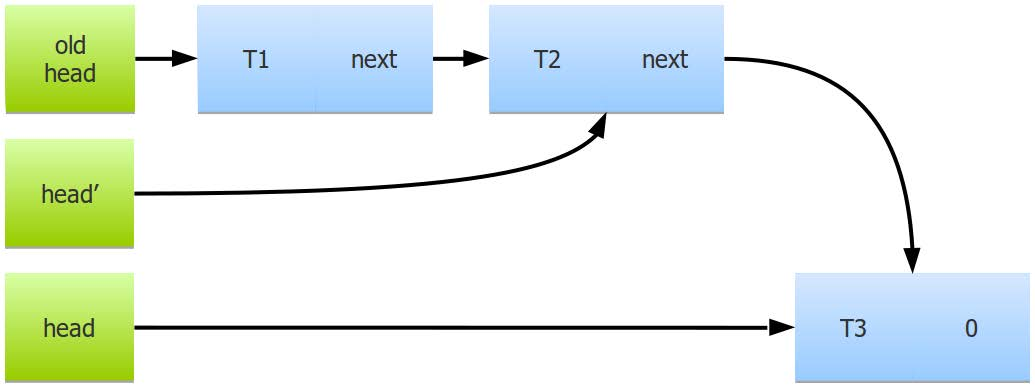
\includegraphics[width=0.9\textwidth]{content/2/chapter7/images/28.jpg}\\
Figure 7.28 – Lock-free insertion and removal at the head of a singly-linked list with shared pointers
\end{center}

Thread B has removed both nodes from the list (Figure 7.28), but the memory has not been released. The new node T4 is allocated at some other address, different from the addresses of all currently allocated nodes. Thus, when thread A resumes execution, it will find the new list head different from the old head value; the compare-and-swap will fail, and thread A will attempt the operation again. At this point, it will re-read the head pointer (and get the address of the node T3). The old value of the head pointer is now gone; since it was the last shared pointer pointing to the node T1, this node has no more references and is deleted. Similarly, node T2 is deleted as soon as the shared pointer head' is reset to its new intended value (the next pointer of the node T3). Both nodes T1 and T2 have no shared pointers pointing to them, so they are finally deleted. 

Of course, this takes care of the insertion at the front. To allow insertion and removal anywhere, we have to make all pointers to the nodes into shared pointers. This includes the next pointers of all nodes as well as the pointers to nodes that are hidden inside list iterators. Such a design has another major advantage: it takes care of the problems with list traversals (such as search operations) that happen concurrently with insertions and deletions.

If a list node was removed while there is an iterator pointing to this list (Figure 7.29), the node remains allocated, and the iterator is valid. Even if we remove the next node (T3), it will not be deallocated because there is a shared pointer pointing to it (the next pointer of node T2). The iterator can traverse the entire list.

\hspace*{\fill} \\ %插入空行
\begin{center}
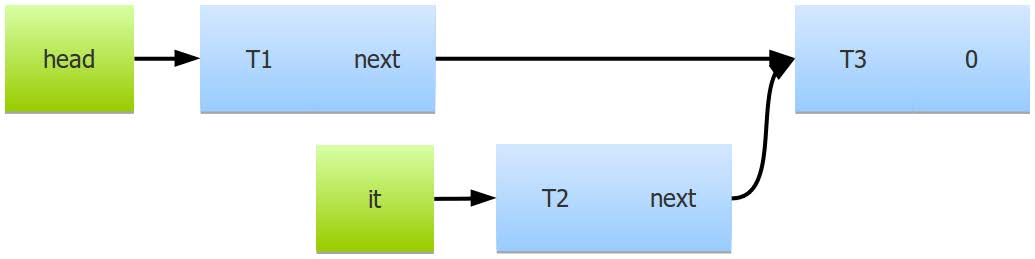
\includegraphics[width=0.9\textwidth]{content/2/chapter7/images/29.jpg}\\
Figure 7.29 – Thread-safe traversal of a lock-free list with atomic shared pointers
\end{center}

Of course, this traversal may include nodes that are no longer in the list, that is, no longer reachable from the head of the list. This is the nature of the concurrent data structures: there is no meaningful way to talk about the current content of the list: the only way to know the content of the list is to iterate over it from the head to the last node, but, by the time the iterator reached the end of the list, the previous nodes might have changed, and the result of the traversal is no longer current. This way of thinking takes some getting used to. 

We are not going to show any benchmarks of the lock-free list versus a lock-guarded list because these benchmarks must be specific to the application. If you benchmark only insertions and deletions at the head of the list (push\_front() and pop\_front()), the spinlock-guarded list will be faster (atomic shared pointers are not cheap). On the other hand, if you benchmark simultaneous insertions and searches, you can make the lock-free list faster by as much as you want: do a traversal of a list of 1M elements with the lock-guarded list locked the entire time while the lock-free list can do simultaneous iterations on every thread, along with insertions and deletions. No matter how slow the atomic pointers are, the lock-free list will be faster if you just make it long enough. This is not a gratuitous observation: your application may need to do the operations that would require locking the list for a very long time unless you can somehow partition the list in a way that avoids deadlocks. If this is what you need to do, the lock-free list is the fastest by far. On the other hand, if you need to iterate over just a few elements and never in many different locations at the same time, a lock-guarded list will do fine. 

The A-B-A problem and the solutions we have listed apply not just to the lists but to all nodal data structures: doubly-linked list, tree, and graph. In data structures linked by multiple pointers, you may encounter additional problems. First of all, even if all pointers are atomic, changing two atomic pointers one after the other is not an atomic operation. This leads to temporary inconsistencies in the data structure: for example, you may expect that going from a node to the next node and back to the previous node will get you back to the original node. This is not always true in the case of concurrency: if a node is inserted or removed at this location, one of the pointers may be updated before the other. The second problem is specific to shared pointers or any other implementation that uses reference counting: if the data structure has pointer loops, the nodes in the loop do not get deleted even when there are no more external references to them. The simplest example is the doubly-linked list, where two adjacent nodes always have pointers to each other. The way we solve this problem in single-threaded programs is by using weak pointers (in a doubly-linked list, all next pointers could be shared, and all previous pointers would then be weak). This does not work as well for concurrent programs: the whole point is to delay the deallocation of memory until there are no more references to it, and the weak pointers do not do that. For these cases, additional garbage collection may be necessary: after the last external pointer to a node is deleted, we have to traverse the linked nodes and check whether there are any external pointers to them (we can do it by checking the reference counts). List fragments with no external pointers can be safely deleted. For such data structures, alternative approaches such as hazard pointers or explicit garbage collection may be preferred. The reader should refer to specialized publications on lock-free programming for more information on these methods. 

This concludes our exploration of high-performance data structures for concurrent programming. Let's now summarize what we have learned.













